\documentclass[final]{beamer}

% ====================
% Packages
% ====================

\usepackage[T1]{fontenc}
\usepackage[utf8]{luainputenc}
\usepackage{lmodern}
\usepackage[size=custom, width=122,height=91, scale=1.2]{beamerposter}
\usetheme{gemini}
\usecolortheme{msu}
\usepackage{graphicx}
\usepackage{booktabs}
\usepackage{tikz}
\usepackage{pgfplots}
\pgfplotsset{compat=1.14}
\usepackage{anyfontsize}

% ====================
% Lengths
% ====================

\newlength{\sepwidth}
\newlength{\colwidth}
\setlength{\sepwidth}{0.025\paperwidth}
\setlength{\colwidth}{0.3\paperwidth}

\newcommand{\separatorcolumn}{\begin{column}{\sepwidth}\end{column}}

% ====================
% Title
% ====================

\title{From Sentiment to Signals: FinMini LLM for Financial Sentiment Analysis and Text-Driven Stock Movement Prediction}

\author{JiaYi Zhang \and JiaYuan Jiang \and Yue Yu \and YiXiang Fei}

\institute[UMich]{Electrical Engineering and Computer Science, University of Michigan \quad $\cdot$ \quad EECS 545: Machine Learning}

% ====================
% Footer
% ====================

\footercontent{
  EECS 545 --- Machine Learning \hfill
  University of Michigan, April 2026 \hfill
  \href{mailto:jiayuanj@umich.edu}{jiayuanj@umich.edu}}

% ====================
% Logo
% ====================

\logoright{\includegraphics[height=5cm]{logos/blockM.png}}

% ====================
% Body
% ====================

\begin{document}

\begin{frame}[t]
\begin{columns}[t]
\separatorcolumn

% ==================== COLUMN 1 ====================
\begin{column}{\colwidth}

  \begin{block}{Motivation}

    [TODO: motivation content]

  \end{block}

  \begin{block}{Problem Statement}

    [TODO: problem statement content]

  \end{block}

  \begin{block}{Related Work}

    [TODO: related work content]

  \end{block}

\end{column}

\separatorcolumn

% ==================== COLUMN 2 ====================
\begin{column}{\colwidth}

  \begin{block}{Approach}

    \heading{Two-Stage Fine-Tuning Pipeline}

    [TODO: pipeline figure and description]

    \heading{Base Model and Fine-Tuning Method}

    [TODO: DeepSeek-R1-Distill-Llama-8B + QLoRA details]

  \end{block}

  \begin{exampleblock}{Data}

    Fine-tuning quality is bottlenecked by data quality and diversity.
    We select three datasets that balance \textbf{annotation reliability}
    (FPB: 100\% inter-annotator agreement), \textbf{scale} (DS2: 100K+
    multi-source samples), and \textbf{task diversity} (FLARE-SM-ACL:
    market-movement reasoning). Each sample is further augmented via
    \textbf{DeepSeek API} into CoT-SFT format --- replacing bare labels
    with structured \texttt{<think>}\ldots\texttt{</think>} reasoning
    traces --- producing interpretable, reasoning-rich training signal
    aligned with DeepSeek-R1's native format (Ou \& Yin, 2025).

    \heading{Training Corpus \normalfont\small(63,395 train / 7,979 test)}

    \begin{table}
      \centering
      \small
      \begin{tabular*}{\linewidth}{@{\extracolsep{\fill}}lrp{0.44\linewidth}}
        \toprule
        \textbf{Dataset} & \textbf{Size} & \textbf{Selection Rationale} \\
        \midrule
        FPB          &  2,264  & 100\% inter-annotator agreement; highest label quality \\[0.4ex]
        DS2          & 100,037 & Multi-source aggregation (FinGPT, Twitter); provides scale \\[0.4ex]
        FLARE-SM-ACL &  27,056 & Market reasoning beyond sentiment; multimodal signal \\
        \bottomrule
      \end{tabular*}
    \end{table}

    \heading{Evaluation Benchmarks}

    \begin{table}
      \centering
      \small
      \begin{tabular*}{\linewidth}{@{\extracolsep{\fill}}llrl}
        \toprule
        \textbf{Benchmark} & \textbf{Task} & \textbf{Size} & \textbf{Split} \\
        \midrule
        en-FPB      & Sentiment (news)    &   393 & In-dist.  \\
        FiQA-SA     & Sentiment (Q\&A)    &   217 & Unseen    \\
        SM-BigData  & Stock movement      & 1,472 & Unseen    \\
        SM-CIKM     & Stock movement      & 1,143 & Unseen    \\
        \bottomrule
      \end{tabular*}
    \end{table}

  \end{exampleblock}

\end{column}

\separatorcolumn

% ==================== COLUMN 3 ====================
\begin{column}{\colwidth}

  \begin{block}{Results and Evaluation}

    \heading{Training Convergence}

    We fine-tune DeepSeek-R1-Distill-Llama-8B with QLoRA on 63K samples
    for one epoch (${\sim}16$K steps). Cross-entropy loss decreases steadily
    from ${\sim}3.0$ to ${\sim}1.75$, confirming stable convergence without
    overfitting.

    \begin{figure}
      \centering
      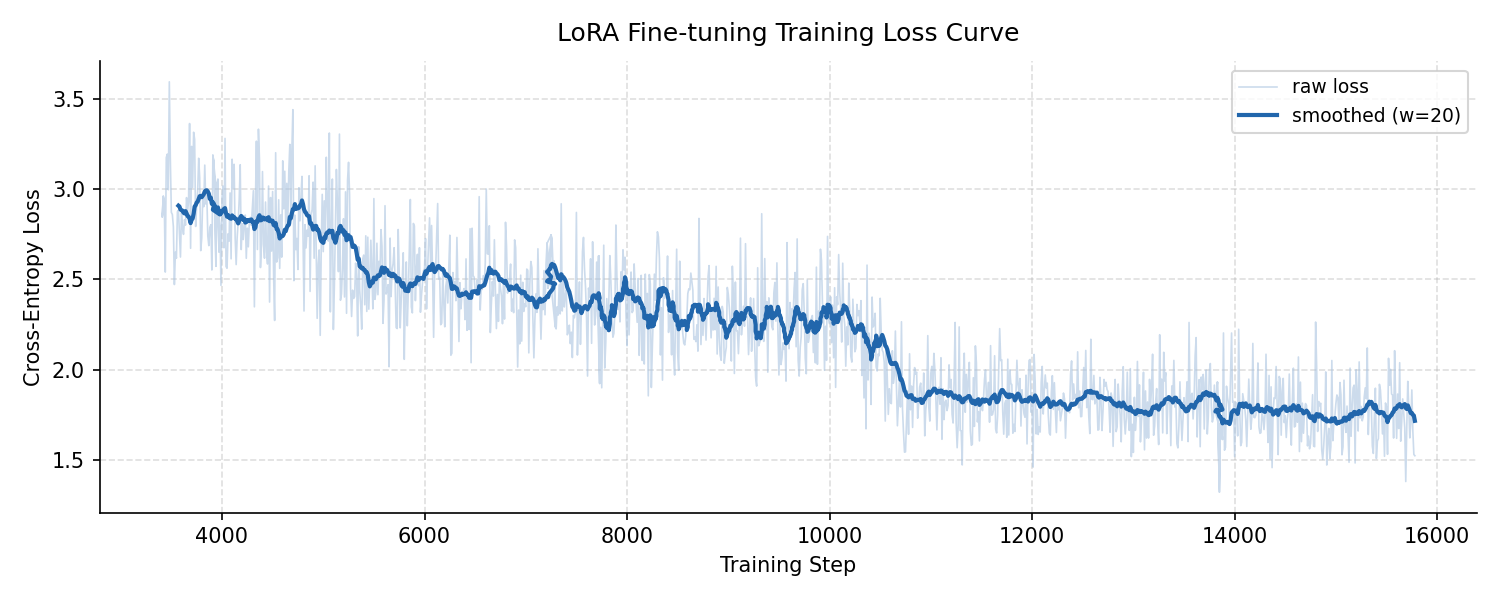
\includegraphics[width=0.85\textwidth]{figures/fig5_training_loss.png}
    \end{figure}

    \heading{Accuracy on Open FinLLM Benchmarks}

    We evaluate on four benchmarks from the Open FinLLM Leaderboard:
    FPB (news sentiment), FiQASA (Q\&A sentiment), SM-BigData and SM-CIKM
    (stock movement prediction).
    FinMini achieves the best accuracy on all four tasks.
    Gains are largest on sentiment benchmarks (+9.6\% on FPB, +12.5\% on FiQASA
    over the strongest baseline), while stock movement tasks also improve,
    confirming that domain fine-tuning generalizes across financial NLP.

    \begin{figure}
      \centering
      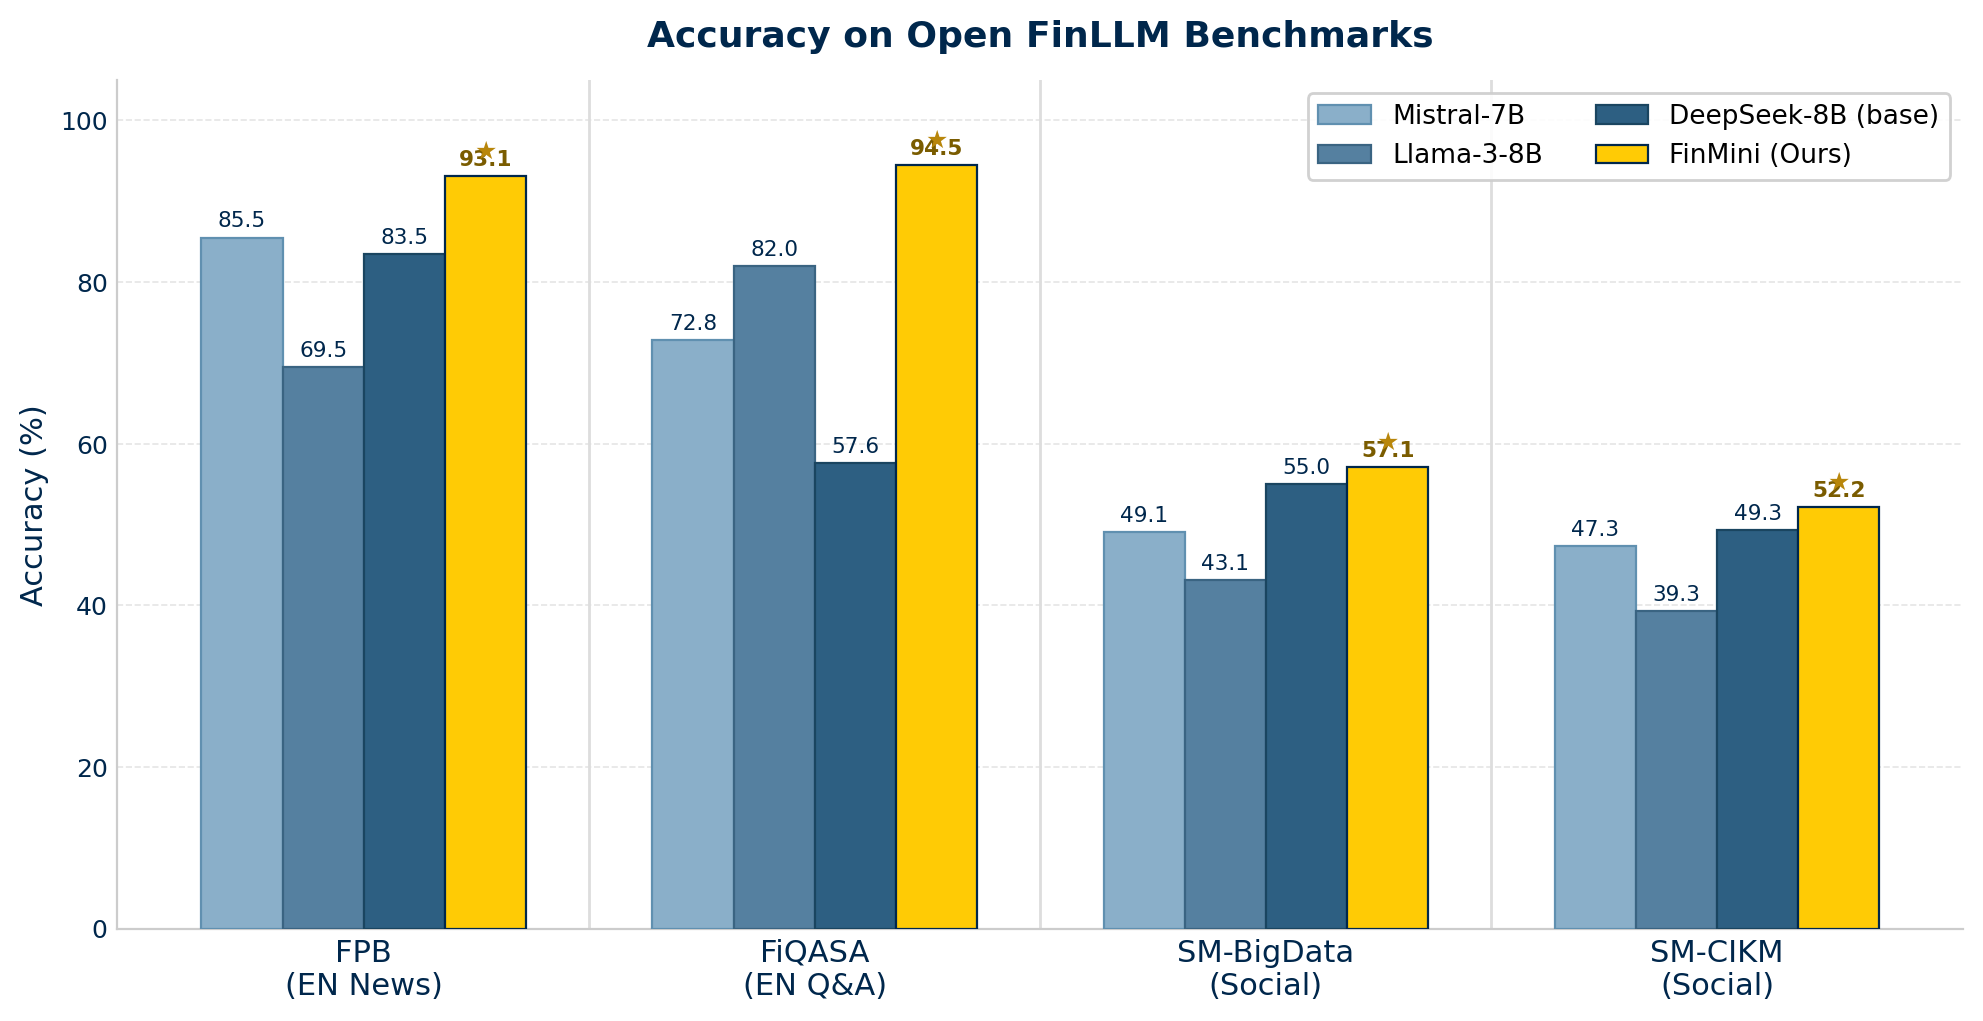
\includegraphics[width=\textwidth]{figures/fig7_bar.png}
    \end{figure}

  \end{block}

  \begin{alertblock}{Conclusion}

    [TODO: conclusion bullet points]

  \end{alertblock}

  \begin{block}{References}

    \scriptsize
    \setlength{\parskip}{0.3ex}
    \noindent
    [1] Ou \& Yin. \textit{Empowering Lightweight MLLMs via Long CoT SFT}. arXiv:2509.03321, 2025.

    \noindent
    [2] Araci. \textit{FinBERT: Financial Sentiment Analysis with Pre-trained LMs}. arXiv:1908.10063, 2019.

    \noindent
    [3] Xie et al. \textit{PIXIU: A Large Language Model and Benchmark for Finance}. NeurIPS, 2023.

    \noindent
    [4] Wu et al. \textit{BloombergGPT: A Large Language Model for Finance}. arXiv:2303.17564, 2023.

    \noindent
    [5] Huang et al. \textit{Open-FinLLMs: Open Multimodal LLMs for Financial Applications}. arXiv:2402.04616, 2024.

  \end{block}

\end{column}

\separatorcolumn
\end{columns}
\end{frame}

\end{document}
